\section{Analysis}
\subsection{Problem Defenition}
This project aims to produce a user-friendly means to interact with the SpaceTraders API, an online space trading game that uses http requests to communicate with the server and manage a fleet of ships, however that lacks a frontend client for users to interact with. The core gameplay loop revolves around accepting loans, and performing mining operations to gather the required resources to repay those loans. Credits can then be used to improve your fleet and in turn, increase one's mining capacity – allowing larger loans to be taken for more credits.

To play Space Traders you must first register yourself a callsign e.g. (L3O, TR4D3R etc..) which identifies an agent. Contracts, ships, and credits are all associated with an agent identity. The Space Traders universe is composed of systems and waypoints. Waypoints are locations within a system such as a planet, moon or asteroid, and consist of a type, x-y coordinates, and set of features such as a shipyard or marketplace. Ships can navigate between waypoints or warp between systems. An agent earns credits by taking contracts with a deadline and requirements for completion e.g. (deliver "205 IRON\_ORE" to destination: "X1-QT13-H53" by "2024-03-15T12:04:25.707Z"). 

To complete a mining contract, you must locate an asteroid containing the required ore, and send your purchased mining droid to mine the resource. Cargo can then be sold at marketplaces to earn credits and offload cargo, with variable market rates for each resource depending on the volume being traded; which affects both the stability and magnitude of the market price. 

Since SpaceTraders lacks a frontend for users to interact with, actions are performed via http requests sent to the Space Traders server. For example, this request to navigate to the waypoint X1-QT13-H53:
\begin{lstlisting}
curl --request POST \
 --url 'https://api.spacetraders.io/v2/my/ships/L30_DE-1/navigate' \
 --header 'Authorization: Bearer eyJ[...]pQw' \
 --header 'Content-Type: application/json' \
 --data '{
    "waypointSymbol": "X1-QT13-H53"
   }'
\end{lstlisting}
My project will be to produce a frontend client to interact with the Space Traders API in a user-friendly manner, and will be targeted towards someone with at least a basic understanding of the command line – thus comfortable using commands to manage their fleet. However new to the game of Space Traders. 

\subsection{Programming Language}
The first decision to make regarding to this project is that of programming language – more specifically a choice between two stable, statically typed languages with strong module support and asynchronous runtimes. Go and Rust. The former (renowned for its simplicity and concurrency) would offer an expediated development cycle with an extensive standard library. Rust, however, offers memory safety, performance and a strict typing system – enforcing good programming practices. In addition to a superior multiplatform bundler for distributing the program as a single binary without dependencies. Furthermore, Rust has a more mature and documented ecosystem for Terminal User Interfaces (TUI) and Command Line Interfaces (CLI) – which I intend to explore as a means for the user to interact with the API. Below is the same program demonstrating registration with the SpaceTraders API written in Rust and Go respectively to illustrate their differences. 

\subsubsection{Prototyping}
The prototypes below go through the process of registering an agent, and handling any potential http errors – or the case wherin an agent symbol has already been taken. The agent data is stored in a HashMap with attributes corresponding to their respective json keys, and which is later serialised into the body of a http POST request. Both languages use asynchronous programming techniques to ensure the response has been recieved before processing resumes, (\texttt{async} in rust, and \texttt{defer} in go). The response is then deserialised into a HashMap and is checked for errors (in which case the applicable error is neatly printed) – else the agent's token is output to the console and the agent has been registered successfully.
\begin{lstlisting}[language=C]
use std::collections::HashMap;
use reqwest::{Client, Error};

async fn register() -> Result<String, Error> {
    let client = Client::new();

    let agent = HashMap::from([
        ("symbol", "L30_DESILVA"), 
        ("faction", "COSMIC")
    ]);

    let res = client
        .post("https://api.spacetraders.io/v2/register")
        .header("Content-Type", "application/json")
        .json(&agent)
        .send()
        .await?
        .json::<serde_json::Value>()
        .await?;

    if let Some(error) = res.get("error") {
        println!("{}", error["message"])
    } else {
        println!("Congratulations, {}. You have been 
            registered. Please note your token.", 
            res["data"]["agent"]["symbol"]);
        println!("{}", res["data"]["token"]);
    }

    Ok(res["data"]["token"].to_string());
}

#[tokio::main]
async fn main() {
    let _ = register().await.unwrap();
}

\end{lstlisting}

\begin{lstlisting}
$ http_prototype git:(master): cargo run
    Compiling http_prototype v0.1.0 
      Finished dev [unoptimized] target(s) in 0.51s
      Running `target/debug/http_prototype`

Congratulations, "L30_DESILVA". You have been registered.
Please note your token:
"eyJhbGciO[...]QhEdECLg"

$ http_prototype git:(master): cargo run
    Finished dev [unoptimized] target(s) in 0.07s
     Running `target/debug/http_prototype`

"Cannot register agent. Agent symbol L30_DESILVA has already been claimed." 

\end{lstlisting}

The equivalent Go code, due to its simplicity, can be tedious and lengthy to write. 

\begin{lstlisting}[language=C]
package main

import (
	"bytes"
	"encoding/json"
	"fmt"
	"net/http"
)

type Register struct {
    Data map[string]interface{}
    Error map[string]interface{}
}

func main() {
    body, err := json.Marshal(map[string]string{
        "symbol": "TRUCKER",
	    "faction": "COSMIC",
    }) 

    if err != nil {
        panic(err)
    }

    req, err := http.NewRequest(
        "POST",       
        "https://api.spacetraders.io/v2/register", 
        bytes.NewBuffer(body)
    )

    if err != nil {
        panic(err)
    }

    req.Header.Add("Content-Type", "application/json")
    client := &http.Client{}
    res, err := client.Do(req)
    if err != nil {
        panic(err);
    }

    defer res.Body.Close()

    data := Register{}
    err = json.NewDecoder(res.Body).Decode(&data)
    if err != nil {
        panic(err)
    }

    if len(data.Error) != 0 {
        fmt.Println(data.Error["message"])
    } else {
        var agent map[string]interface{}
        agentJson, err := json.Marshal(data.Data);
        if err != nil {
            panic(err)
        }

        err = json.Unmarshal(agentJson, &agent);
        if err != nil {
            panic(err)
        }

        fmt.Printf("Congratulations, You've been successfully registered. Please note your access token:\n")
        fmt.Println(agent["token"])
    }
}
\end{lstlisting}

Due to its stability, performance, security and mature, centralised ecosystem I will use rust for this project. Although Rust’s somewhat convoluted approach to asynchronous programming will require careful design considerations as to not introduce bugs. And it's combination of a restrictive borrow checker and strict compiler enforces good programming practices and memory safety, with verbose handling of all potential errors mitigting the risk of crashes and ensuring programs are always stable, performant and reliable. 

\subsection{API}
A web API (Application Programming Interface) is a set of standard protocols to interact with a web server. The Space Traders API offers HTTP end-points with which programs can access, and in turn: play the open universe trading game. Actions are performed via http requests to the Space Traders server, and such actions can range from locating all available shipyards in a system (\textcite{spacetraders}):
\begin{lstlisting}
curl 'https://api.spacetraders.io/v2/systems/:systemSymbol/waypoints?traits=SHIPYARD' --header 'Authorization: Bearer INSERT\_TOKEN\_HERE'
\end{lstlisting}
To selling ship cargo:

\begin{lstlisting}
curl --request POST \
 --url 'https://api.spacetraders.io/v2/my/ships/:miningShipSymbol/sell'
 --header 'Authorization: Bearer INSERT_TOKEN_HERE' \
 --header 'Content-Type: application/json' \
 --data '{
    "symbol": "IRON_ORE",
    "units": "100"
   }'
\end{lstlisting}

However, there are 2 versions of the SpaceTraders API in production, the complete V1, and the alpha V2 release. The former is more stable due to its maturity, and has a wider variety of available resources: including frontend clients and tutorials to learn from. Yet it lacks much of the expanded functionality of the second release and is no longer actively maintained. Whereas V2 consists of a larger universe, a wider breadth of expanded features, and more comprehensive documentation. (\textcite{spacetraders}) Thus, my project will utilise the V2 API specification albeit hesitant of potential bugs due to the alpha nature of its release. 

\subsection{Existing Systems}
There are various existing frontends that use either a command line interface (CLI), or a graphical user interface (GUI) to interract with the SpaceTraders API. A command line interface (as illustrated below) allows for expediated development, however can appear confusing, intimidating, and untintuitive without experience, wheras a GUI whilst visually intuitive, offers less flexibility and a slower development cycle. A common thread between all clients is the manner in which systems distill the complex http queries into a simpler interface when interacting with the server.
\bigskip

\shadowbox{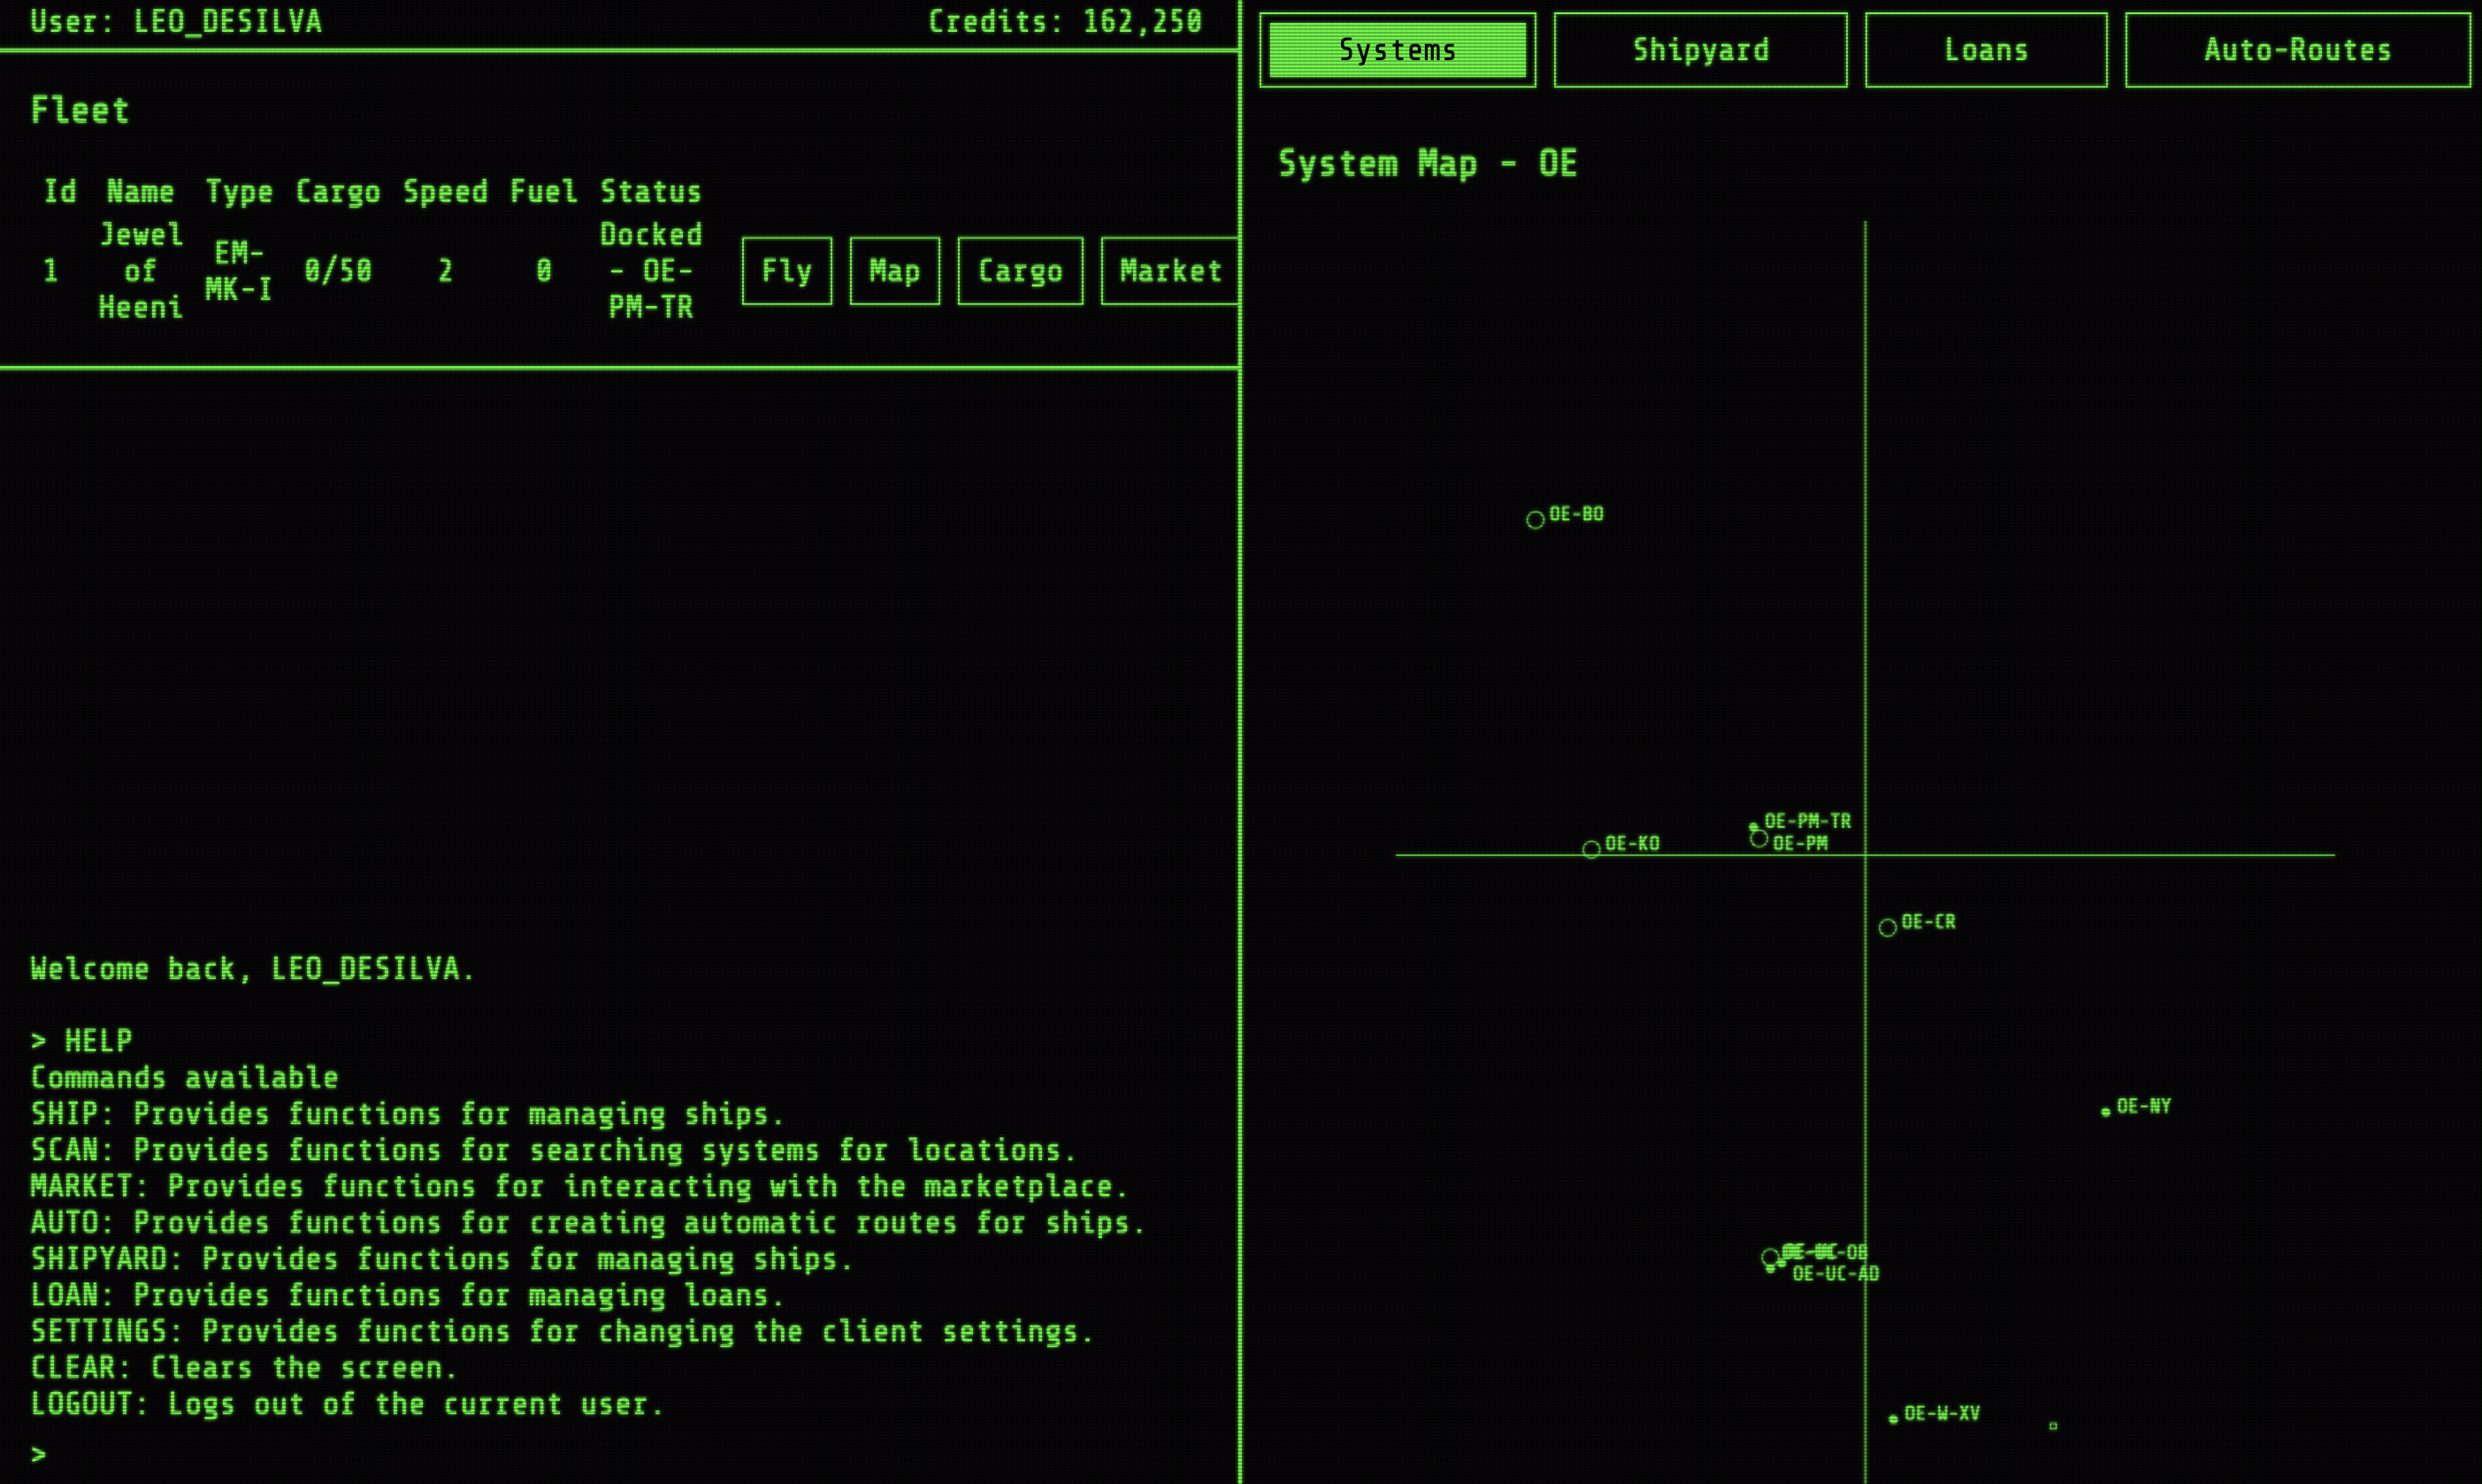
\includegraphics[width=11cm]{trade-commander.png}}

Trade Commander (\textcite{tradecommander}) is a CLI client for the SpaceTraders API that uses a split screen approach where commands are input in the console on the left and their output shown graphically through the display on the right. Trade Commander thus merges the flexibility of textual interfaces with the intuitiveness of a GUI. It offers a dashboard layout where commonly relevant information can be accessed at a glance: such as ones fleet, star map, owed loans, and trade market. This has the advantage of being efficient to use, however comprises a considerable learning curve when initially getting started with Space Traders.  

\bigskip
\shadowbox{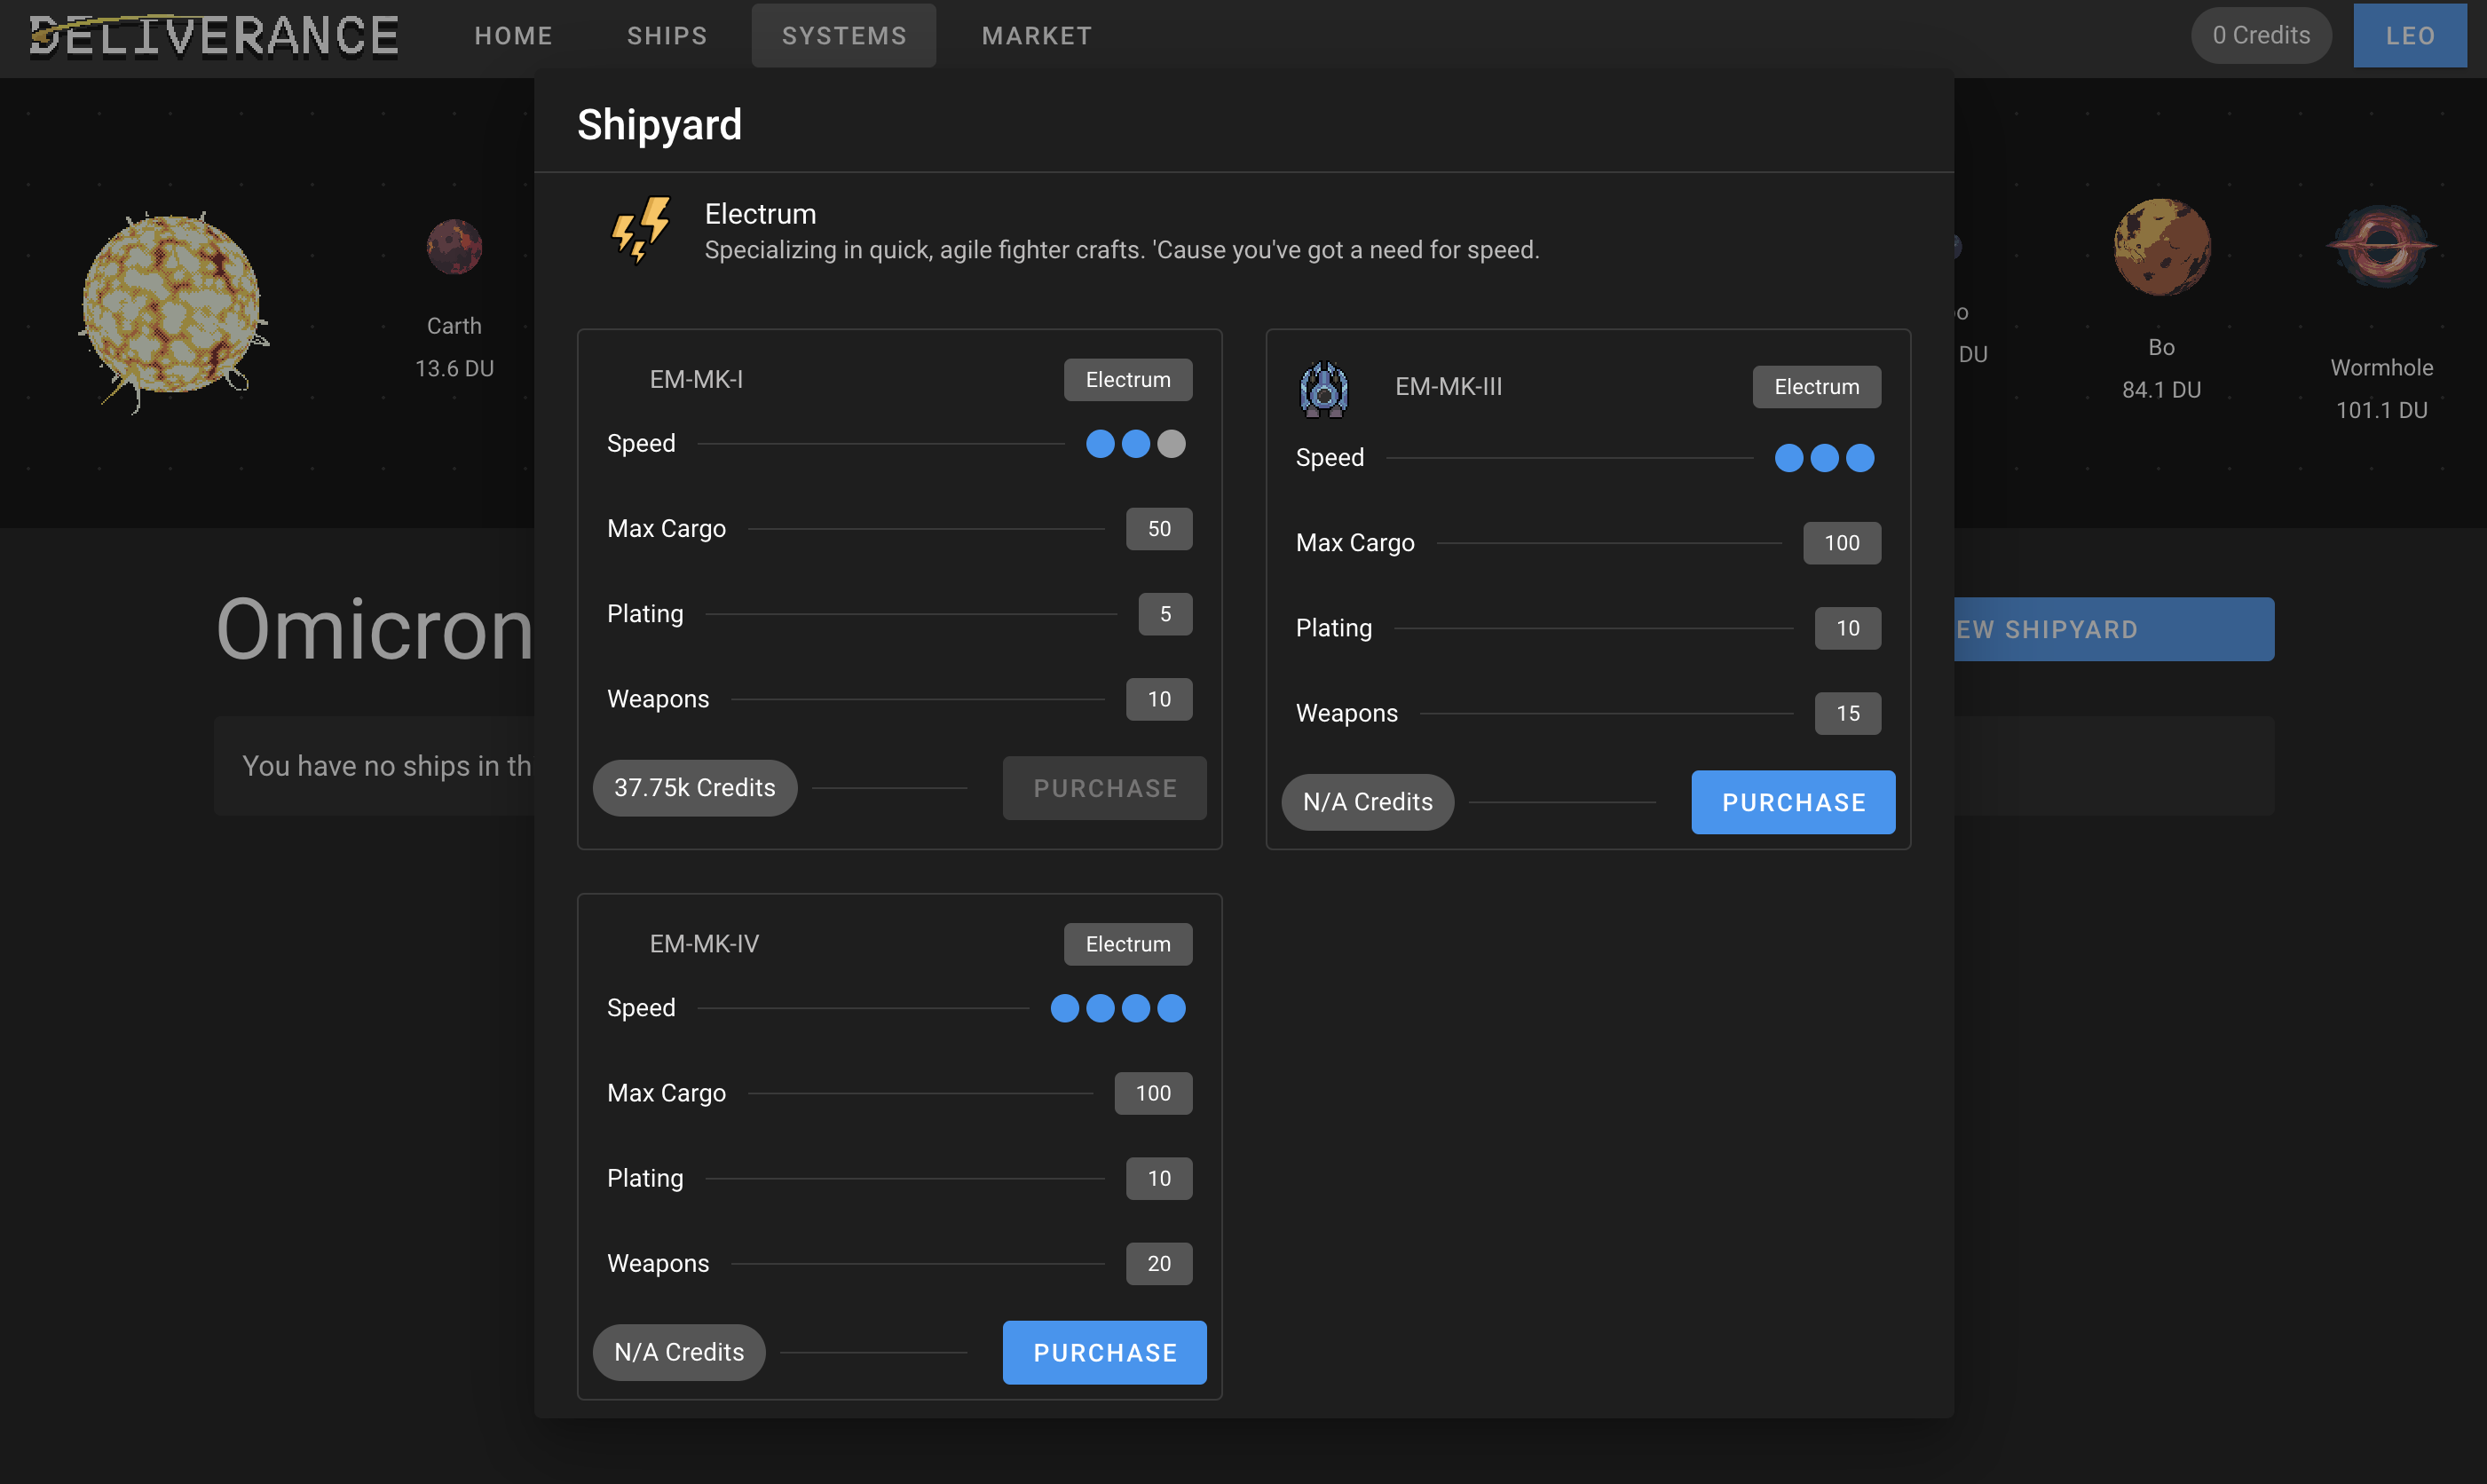
\includegraphics[width=11cm]{deliverance.png}}

Deliverance (\textcite{deliverance}) took a different approach, opting for a graphical UI, synthesising the http requests required to interact with the API into a series of menus and buttons that are intuitive to work with. Stumblinbear has organised the available operations into 4 categories: Home, Ships, Systems, and Market. This has the advantage of being comparatively easy to work with, however will slow down development due to the resources needed to create a graphical interface and limits the flexibility of the system when adding new functionality.

In conclusion, I will look at approaching my frontend similarly to that of Trade Commander, with an interspersion of textual and graphical elements thus utilising the respective advantages of both GUIs and CLIs: allowing for both a simple and easy to understand visualisation of your fleet, and complex commands that can be entered with comparative ease. Furthermore this creates a more 'retro' aesthetic that suits the nature of the game. 

\subsection{Client Proposal}
My client for this project will be someone with at least a basic understanding of the command line, and new to the game of SpaceTraders. The set of features I will propose is as following:
\begin{enumerate}
    \item A Terminal User Interface (TUI) comprising of a command line and graphical interface.
        \begin{enumerate}
            \item The CLI allow the user to input commands and manage their fleet, as well as displaying their respective output in a neatly organised manner. An example use of how one might use the CLI to direct a ship with \texttt{ship\_id: 2} to \texttt{waypoint: X1-QT13-H53} would be \texttt{ship fly --ship\_id 2 --waypoint X1-QT13-H53}
            \item The output of commands will either be communicated textually through the console, or by updating the graphical display. An example command of the former type may be listing all ships present in a particular shipyard, and for the latter – moving between systems will update the star map.
        \end{enumerate}
    \item The ability to register or login to an account using an access token.
        \begin{enumerate}
            \item The user will be welcomed with a prompt to either login to an existing account (by providing their access token), or to create a new account.
            \item Should they opt to create a new account, they will be presented with another prompt to enter their desired agent symbol, and the case wherin a symbol has already been taken will be handled.
        \end{enumerate}
    \item The ability to purchase ships and manage one's fleet through various commands including:
        \begin{enumerate}
            \item Displaying a list of waypoints or systems within reach of a ship - taking into consideration the ship's speed and fuel level.
            \item Navigating between available systems and waypoints, this will take into consideration the fuel of the ship and will update the graphical display to show both the current system/waypoint and previously visited waypoints.
            \item The ability to view the contents of a shipyard, and purchase the desired ship with credits. 
        \end{enumerate}
    \item The ability to take out and repay loans.
        \begin{enumerate}
            \item With a command, you will be able to view all availabe loans, their expiration date, resource required, and credits rewarded.
            \item Similarly, you will also be able to accept loans and view your current loan through the graphical interface.
        \end{enumerate}
    \item The ability to manage one's mining operations.
        \begin{enumerate}
            \item You will be able to view the cargo of any paritcular ship, and the being used to carry it. 
            \item Ship's will be able to mine resources from asteroids and add the resource to their cargo – the ship exceeds its weight limit.
            \item You will be able to sell cargo at various markets throughout the universe for market prices and collect the credits.
        \end{enumerate}
    \item The ability to visually display a map of the star system.
        \begin{enumerate}
            \item The graphical display will show the current system and all of its waypoints, as well as indicating the locations of any ships in your fleet and previously visited locations.
        \end{enumerate}
\end{enumerate}

My system will use integrate aspects of both a CLI and GUI. The console permits the flexibility of input that is limited by a GUI, and the graphical interface can display the results of such commands or other relevant information to the user, including but not limited too: a map of the star system, the progress of ongoing mining operations, any pending loans etc... My system will include means of querying data from the API which can be sorted and displayed according to the user's requirements, such as ordering loans by their reward, or displaying all unsold ships in the system. 

\subsubsection{Client Interview}
I will interview my client about their experience playing Space Traders, and gather their thoughts on the frontends they have used. Here are the questions I intend to ask:
\begin{enumerate}
    \item Have you ever played a game of Space Traders? \\
        \textit{"I have played through the tutorial, to get an idea of what the game is. But I'm not a regular player. I still don't understand how most of the systems actually work.}
    \item Which features of your client(s) did you like? \\ 
        \textit{"I'm already pretty used to a command line, so I liked how quick it was to anything done. There was a command for everything, and they displayed the results in a nice and organised manner (2.2, 2.3). I also thought the design suited nature of the game pretty well – like one of those 80's text adventure games with the green and black terminal font. (1.1.1)"}
    \item Which features of your client(s) did you dislike? \\ 
        \textit{"I didn't like how difficult it was to get started, the HELP command didn't even list all the available commands, I needed to have the documentation open on the side to get anywhere! I also didn't like how it made you input your token for every single request. (2.1.1)"}
    \item Which part of the game did you find the most difficult to understand? And what could have helped you understand it better?\\
        \textit{"I still don't understand how complicated it is to get anywhere, you have to set a flight mode, dock your ship – and it becomes tedious to get anywhere in a reasonable time. (2.3.1)" }
    \item Did you find a graphical interface improved your understanding of the game?\\
        \textit{"I liked seeing the place's I'd been, and it gave a nice visual way of seeing how far i'd come since I started. Although I found that just the starmap was a little dull, especially when it was nearly empty. I liked how the view changed based on different commands, like to show the available ships or loans. (1.3)"}
    \item Would you have found a tutorial system beneficial to your enjoyment when first starting out with Space Traders? \\
        \textit{"I think SpaceTraders own tutorial is pretty overwhelming, but if the frontend is well intuitive its pretty maneagable. I think the main thing is, especially when you're using a CLI, having a quick breakdown of all the comamnds you can use, and the parameters they require goes a long way."}
    \item Which of the above clients appeals the most to your tastes? And what did you like about it?\\
        \textit{"I mean, I used the second one because I liked the way it looked. But it's quite unstable and opaque. I think if i'd started with the first one I might've understood the game a little better."}
\end{enumerate}

\subsection{Objectives}
\begin{enumerate}
    \item \textbf{Interface \& Interaction}
    \begin{enumerate}
        \item The program should run as a Terminal User Interface (TUI). (\textit{1.4 Existing Systems})
            \begin{enumerate}
                \item The program should be designed in the style of an 80's text adventure game with textual interfaces.
            \end{enumerate}
        \item A CLI console should be used to enter commands and manage one's fleet. (\textit{1.4 Existing Systems})
            \begin{enumerate}
                \item The program should be able to take, sanitise and process user input, distilling it into a series of http requests required to complete the desired task. 
                \item The program should be able to serialise the results of such requests and communicate any relevant information textually to the user through the console.
            \end{enumerate}
        \item Information regarding the star system and ongoing operations should be communicated both textually and through a graphical interface. (\textit{1.5.1 Client Interview})
            \begin{enumerate}
                \item The graphical display should show a map of visited waypoints, as well as information about the current waypoint.
            \end{enumerate}
        \item The program should support the SpaceTraders V2 API specification (\textit{1.3 API})
    \end{enumerate}

    \item \textbf{Functionality}
    \begin{enumerate}
        \item Users should be able to register a new agent, or login to an existing agent with an API token. (\textit{1.1 Problem Defenition})
            \begin{enumerate}
                \item Should the user register a new agent, the program should store their API token to streamline future requests.
                \item A prompt should be shown for the user to enter their agent symbol and the program should handle the case wherin a symbol is already taken.
            \end{enumerate}
        \item Users should be able to takeout and repay their loans as well as viewing their existing loans through the console. (\textit{1.1 Problem Defenition})
            \begin{enumerate}
                \item When queried, a textual list of all available loans with their respective reward and resource required should be shown. \texttt{loans --list}
                \item The user should be able to take out a loan, and repay such a loan through a series of console commands. 
                \item The resource required, and reward for completion of the current loan should be displayed to the user with a single command. \texttt{loans repay --loan\_id 0 -- resource IRON\_ORE --ammount 5}
            \end{enumerate}
        \item Users should be able to manage their fleet, browse, and purchase ships as well as carrying out mining operations. (\textit{1.1 Problem Defenition})
            \begin{enumerate}
                \item Users should be able to navigate \& dock their ships to a waypoint as well as viewing a list of all waypoints within warping distance with the current fuel level through commands such as \texttt{ship set-flight CRUISE --ship\_id 2} or \texttt{waypoints --list}.
                \item Users should be able to list the contents of a particular shipyard when docked there – and view with a brief overview of the price, speed, defences, weapons and capacity of any ships.
                \item Users should be able to purchase a ship from a shipyard and manage the state of all the ships in their fleet.
            \end{enumerate}
        \item Users should be able to view a visual map of the star system \& visited waypoints. (\textit{1.5.1 Client Interview})
            \begin{enumerate}
                \item The display must show the state of your current system with a bolder marker  used to indicate a waypoint with a ship present, a dim grey marker an unexplored waypoint, and a lighter grey waypoint a previously visited one.
            \end{enumerate}
    \end{enumerate}
    \end{enumerate}

\subsection{Data Modelling}
Maintaining program state through a series of compound data structures – representing various aspects of the system such as an agent, ship or loan - is vital to creating a program that achieves the objectives outlined above. JSON responses from http queries, must be parsed into organised structs with which the program can interact through a series of predefined methods \& public attributes. Structs must be created for Loans, Ships, Agents, Waypoints, \& Systems, the struct for the Agent class might be as described below:
\begin{lstlisting}
Agent:
    * The agent's API access token.
    * An array of the agent's previously visited waypoints.
    * The agent's current loan ID \& resource required for completion.
    * The ID's of all the agent's owned ships.
    * The number of credits possessed by an agent.
\end{lstlisting}
A similar description for the ship, and waypoint class would be as follows:
\begin{lstlisting}
Ship:
    * The ship's flight mode (CRUISE, BURN, DRIFT, STEALTH).
    * The ship's waypoint marker.
    * The ship's current fuel level.
    * The ship's current cargo.
    * The ship's maximum weight, and the current weight of cargo.

Waypoint:
    * The waypoint's x,y coordinates.
    * The waypoints symbolic name.
    * Traits for that particular waypoint e.g. (MARKETPLACE, SHIPYARD).
\end{lstlisting}
There will be a \texttt{GameState} struct containing references to the objects defined above, and will be passed by reference as a parameter to functions, in turn, managing the state of the program through the centralised structure. 